\chapter{Introduction}\label{ch:introduction}
\justify

The Open-source Intelligence Data Mining System (OSINT), as is depicted in Figure~\ref{fig:CTraceOSINTSoftware}, is a newly developed sophisticated tool for a law enforcement agency, like the police department, to track theft and trafficking with the help of a precise analysis of call data records (CDRs) and tower dump data.Alongside the police, the one thing that this program needs is to gain huge data sets of the phone stuff and these huge sets that are cumulated are then finally processed and the results retrieved.

\begin{figure}
    \centering
    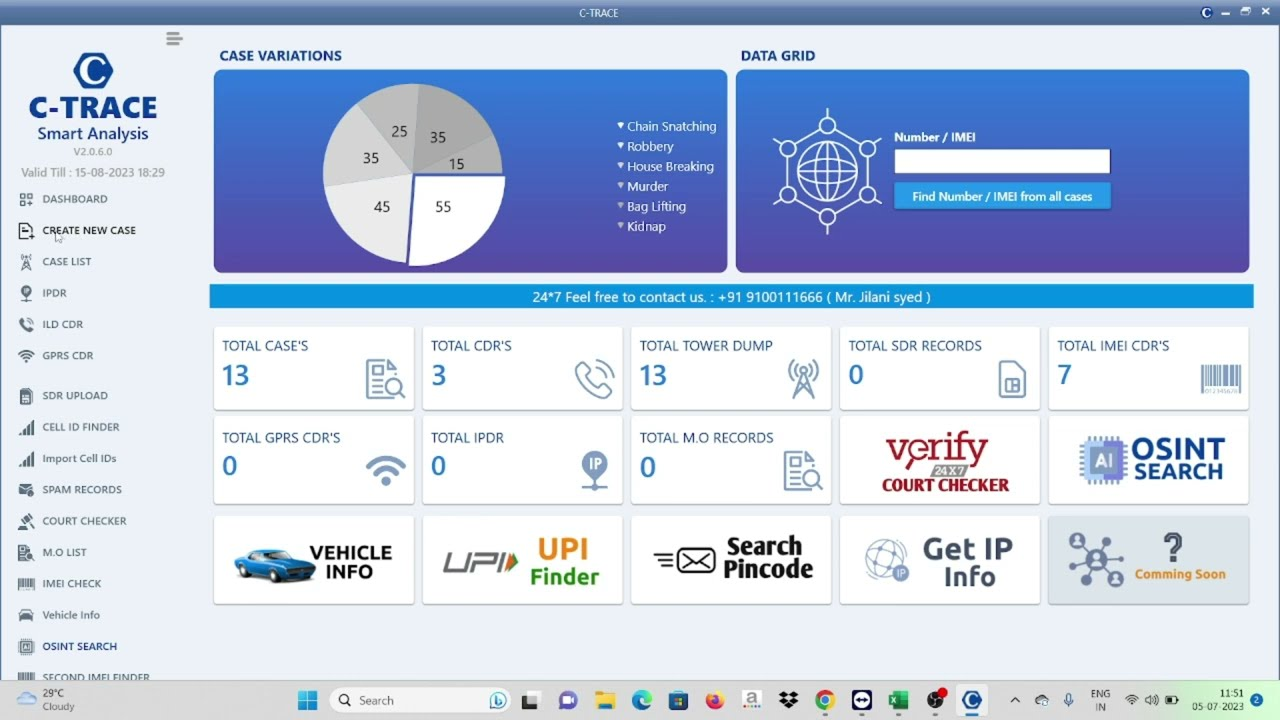
\includegraphics[width=1\linewidth]{Media/maxresdefault}
    \caption{C-Trace OSINT Software}
    \label{fig:CTraceOSINTSoftware}
\end{figure}

This is an application of the method to provide law enforcement agencies with a fast and quick way to analyze call data records (CDRs) and tower dump data.
C-Trace OSINT software is a value-add for investigators as they receive a good number of options for decision making, which in turn is a major progression in their case investigation.


\section{What is the purpose of C Trace's OSINT Software ?}\label{sec:what-is-the-purpose-of-c-trace's-osint-software-?}

C Trace's OSINT (Open Source Intelligence) software is designed to meet the specific needs of law enforcement agencies, particularly the police. The primary purpose of this software is to gather comprehensive information about suspects, which is crucial for police investigations.

Police officers often face restrictions when attempting to obtain data directly from companies. For example, while telecom operators may provide the name of the person who purchased a SIM card, they may not be able to provide information about the actual user of the SIM. This limitation can hinder investigations.

C Trace's OSINT software overcomes these restrictions by providing detailed information without such limitations. It offers:

\begin{itemize}
    \item \textbf{Identification of Actual SIM Users:} The software can reveal the names of the actual users of SIM cards, not just the buyers.
    \item \textbf{Social Media Accounts and Bank Information:} It can provide access to suspects' social media accounts and bank details.
    \item \textbf{Leaked Information on the Internet:} The software also scours the internet for any leaked information related to the suspects.
\end{itemize}

\section{Problems solved with OSINT Software ?}\label{sec:problems-solved-with-osint-software-?}

\begin{itemize}
    \item \textbf{Access Restrictions:} Police face restrictions in obtaining information directly from companies. This software provides the necessary data without such restrictions.
    \item \textbf{Identification of SIM Users:} Telecom operators often provide information about the buyer of a SIM card, but not the actual user. This software identifies the actual SIM users.
    \item \textbf{Comprehensive Data Collection:} It provides access to a wide range of information, including social media accounts and bank details, which are not easily obtainable through conventional means.
    \item \textbf{Leaked Information:} The software can find and utilize leaked information available on the internet, which can be crucial for investigations.
\end{itemize}

\section{What is OSINT Data Mining System ?}\label{sec:what-is-osint-data-mining-system-?}

The application developed is particularly made solely for police as a way to deal with crime by analyzing the call data record (CDR) information and tower dump data only.This tool provides a complex report on people using their phone number, IMEI number, PAN number, and such.It gains tower data, which can show all phone users that are living in a particular tower, by using azimuth ID. The report includes various pieces of information like a person's vehicle particulars, location data, IMEI numbers, phone numbers, PAN numbers, MNP, IP information, etc.And, the software also introduces a PDF that supplies all the necessary data about a person.

\section{Features of OSINT Software}\label{sec:features-of-osint-software}

The developed software provides powerful search functionalities based query.
Below are some of the key features offered:

\begin{enumerate}[label=\textbf{\roman*.}]
    \item \textbf{Vehicle information} : RC MH02ZX1234
    \item \textbf{IP Lookup} : IP 192.168.01.01
    \item \textbf{Pin code search} : PIN 524455
    \item \textbf{IMEI Search} : IMEI 45671234765823 \\
        You can Get Device Model details
    \item \textbf{PNR Search} : PNR 456789101 \\
        Check train ticket status and passenger seat, boarding, and destination info.
    \item \textbf{IFSC Search} : (e.g., IFSC SBIN0062517 or IFSC SBI ATTAPUR) \\
        Find bank details with IFSC code.
    \item \textbf{UPI Search} : UPI 8465802838 \\
        UPI Ids that are linked with a particular mobile number.
    \item \textbf{Court Case Search} : CC Name \\
        Search court cases using the victim name.
    \item \textbf{OSINT Search} : OSINT 9848012345 \\
        Open source Intelligence infomation of UPI IDs, photos, social media accounts, and more.
    \item \textbf{Phone Number to Gas Connection search} : GAS 9848012345
    \item \textbf{Cell ID Search} : BTS 4044349032727 \\
        Tower infomation of a cell ID and active phone numbers under the tower.
    \item \textbf{MNP Lookup} : Network 9848012345 \\
        Get operator information of a mobile number
    \item \textbf{IMEI Last digit finder} : FULL IMEI 45231671101234 \\
        You can identify the last digit of an IMEI number.
\end{enumerate}

\section{Plugins Integrated with C-Trace OSINT Software}\label{sec:plugins-integrated-with-c-trace-osint-software}

This software is integrated with additional tools such as Verify 24x7 Court Checker.
\subsection{Verify 24x7 Court checker}\label{subsec:verify-24x7-court-checker}

Verify 24x7 Court checker - is a third party tool, which keeps a large database of millions of court cases in India along millions of records that are refreshes during the day.


\begin{itemize}
    \item \textbf{Chapter 2:}
    In this chapter, we discuss the tools and technologies used to develop the OSINT software and Call One App.

    \item \textbf{Chapter 3:}
    In this chapter, we discuss the proposed systems and the best systems for OSINT software.

    \item \textbf{Chapter 4:}
    In this chapter, we discuss the architecture of the OSINT software and the Call One application.

    \item \textbf{Chapter 5:}
    In this chapter, we discuss the implementation of Call One, test results, and provide screenshots.

    \item \textbf{Chapter 6:}
    In this chapter, we present the conclusion and future scope of the project.

\end{itemize}

